% ------------------------------------------------------------------------------
% TYPO3 CMS 6.2 LTS - What's New - Chapter "Introduction" (French Version)
%
% @author	Paul Blondiaux <pblondiaux@sodifrance.fr>
% @author	Philippe Herault <philippe.herault@plan-net.fr>
% @license	Creative Commons BY-NC-SA 3.0
% @link		http://typo3.org/download/release-notes/whats-new/
% @language	French
% ------------------------------------------------------------------------------
% Chapter: Introduction
% ------------------------------------------------------------------------------

\section{Introduction}
\begin{frame}[fragile]
	\frametitle{Introduction}

	\begin{center}\huge{Introduction}\end{center}
	\begin{center}\huge{\color{typo3darkgrey}\textbf{(Les faits en bref)}}\end{center}

\end{frame}

% ------------------------------------------------------------------------------
% TYPO3 CMS 6.2 LTS: The Facts (1)
% ------------------------------------------------------------------------------

\begin{frame}[fragile]
	\frametitle{Introduction}
	\framesubtitle{TYPO3 CMS 6.2 LTS : les faits}

	\begin{itemize}
		\item Centrée sur :

			\begin{itemize}
				\item Migration Douce (Smooth Migration)
				\item Des fondements robustes et sécurisés
				\item L'expérience utilisateur
				\item Une interopérabilité/technologie moderne
			\end{itemize}
	\end{itemize}

	\begin{columns}[T]
		\begin{column}{.5\textwidth}
			\begin{itemize}
				\item Release Manager :
				\begin{itemize}
					\item Ernesto Baschny\newline
						ernesto.baschny (at) typo3.org\newline
						Twitter : @baschny
				\end{itemize}
			\end{itemize}
		\end{column}

		\begin{column}{.5\textwidth}
			\begin{figure}
				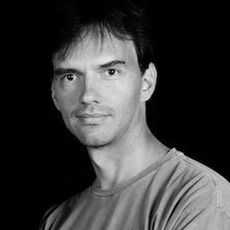
\includegraphics[width=2.6cm,height=2.6cm]{Images/Introduction/ErnestoBaschny.jpg}
			\end{figure}
		\end{column}

	\end{columns}

\end{frame}

% ------------------------------------------------------------------------------
% TYPO3 CMS 6.2 LTS: The Facts (2)
% ------------------------------------------------------------------------------

\begin{frame}[fragile]
	\frametitle{Introduction}
	\framesubtitle{TYPO3 CMS 6.2 LTS: les faits}

	\begin{itemize}
		\item Date de sortie : 25 Mars 2014
		\item Agenda de développement et de sortie :
	\end{itemize}

	\begin{figure}
		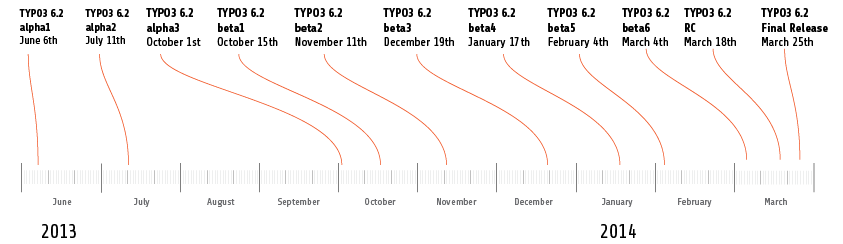
\includegraphics[width=0.99\linewidth]{Images/Introduction/ReleaseTimeline.png}
	\end{figure}

\end{frame}

% ------------------------------------------------------------------------------
% TYPO3 CMS 6.2 LTS: The Facts (3)
% ------------------------------------------------------------------------------

\begin{frame}[fragile]
	\frametitle{Introduction}
	\framesubtitle{TYPO3 CMS 6.2 LTS : les faits}

	\begin{itemize}
		\item Prérequis système
		\begin{itemize}
			\item PHP	\tabto{1.2cm} v5.3.7 - v5.5.x
			\item MySQL	\tabto{1.2cm} v5.1.x - v5.6.x
		\end{itemize}
	\end{itemize}

	\begin{itemize}
		\item Fin de la maintenance : Mars 2017
		\item TYPO3 CMS 6.2 est une version \textbf{Long Term Support} (LTS) (3 ans de support!)
	\end{itemize}

\end{frame}

% ------------------------------------------------------------------------------
% TYPO3 CMS 6.2 LTS: The Facts (4) - Release Agenda
% ------------------------------------------------------------------------------

\begin{frame}[fragile]
	\frametitle{Introduction}
	\framesubtitle{TYPO3 CMS 6.2 LTS : les faits}

	\begin{itemize}
		\item Agenda de sortie :
	\end{itemize}

	\begin{figure}
		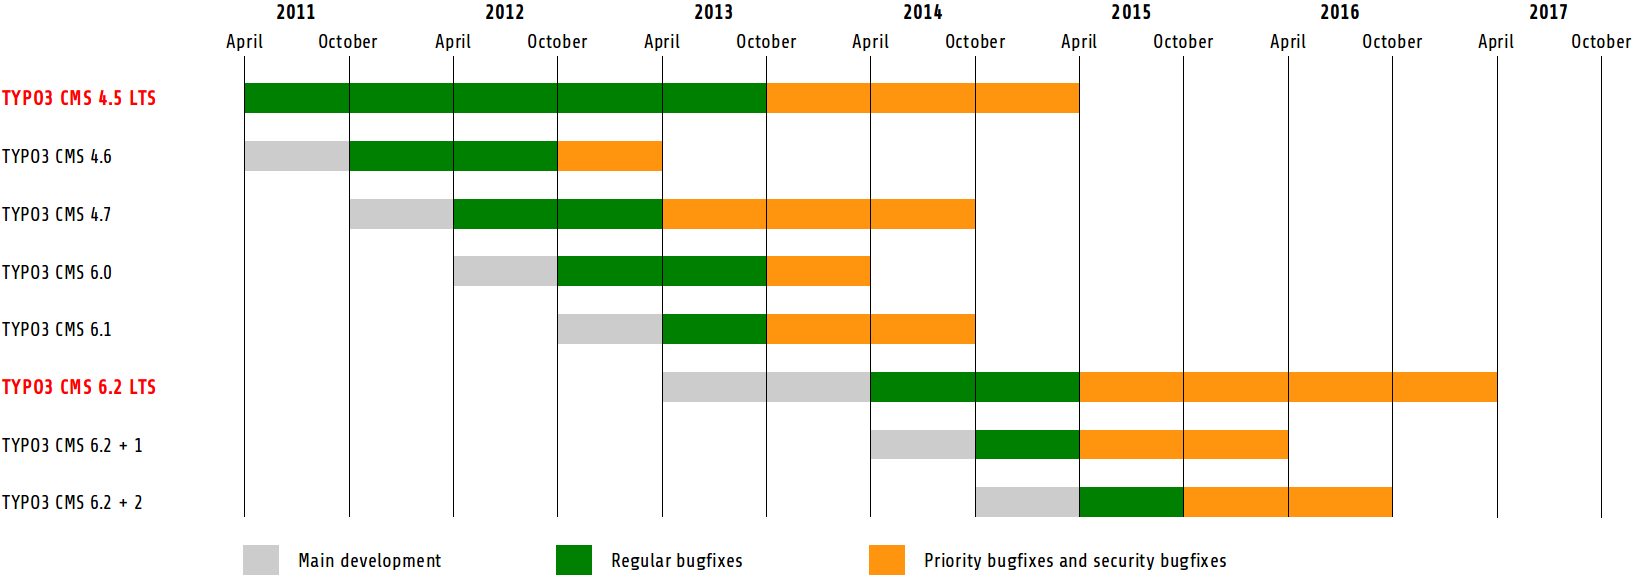
\includegraphics[width=0.99\linewidth]{Images/Introduction/ReleaseAgenda.png}
	\end{figure}

\end{frame}

% ------------------------------------------------------------------------------

